\section{Inverse problem}

Inverse problem in EEG tends to estimate the source by its location and orientation given an instance measurement. This is an ill-posed problem due to its non-unique outcome and highly sensitive to the minor changes (unstable solution) \cite{3}. Two set of methods in solving inverse problem in EEG exist including here, parametric and non-parametric. In this work parametric method is being utilized where it makes an exhaustive search upon a set of initial points for the best fit. The optimization is done iteratively until an arbitrary threshold is achieved. 

\subsection{Estimation of a dipole using a single time instance}

Inverse method has been applied on the on potential distribution outcomed from the dipole located in the coordinates (0.06,0,0.01) oriented along x. The dipole orientation error (DOR) equation \ref{equation_1} and dipole location error (DLE) equation \ref{equation_2} for this particular measurement are outlined in figure \ref{EE1} whereas the RRE plot in figure \ref{RRE1}. From these two figures a consistency of the errors is noted in both these scales for all the five trials. Whereas the potential to be used for this inverse problem is plotted in figure \ref{VO1}.

\begin{figure}[!htbp]
\minipage{0.33\textwidth}%
\centering
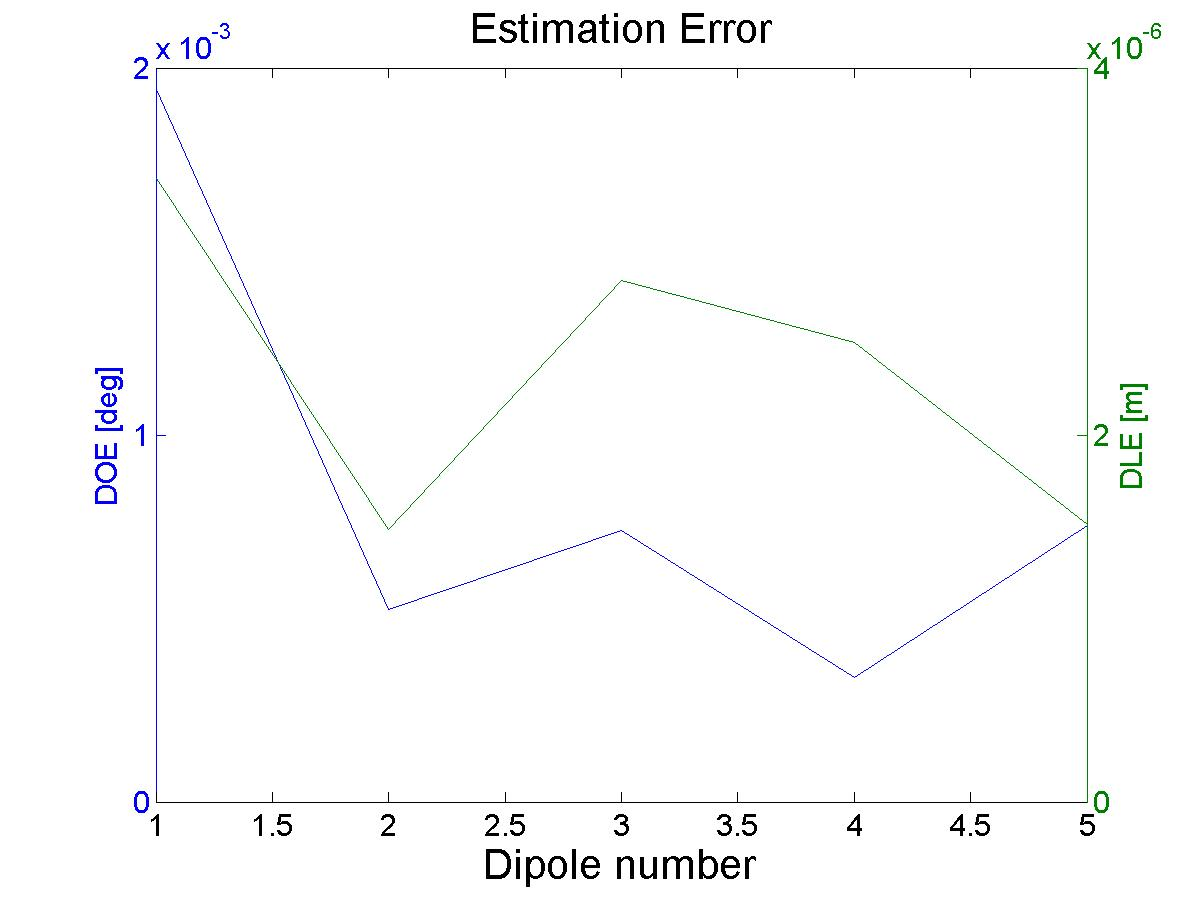
\includegraphics[width=1\linewidth]{100.jpg}
\subcaption{Localisation errors}\label{EE1}
\endminipage\hfill
\minipage{0.33\textwidth}%
\centering
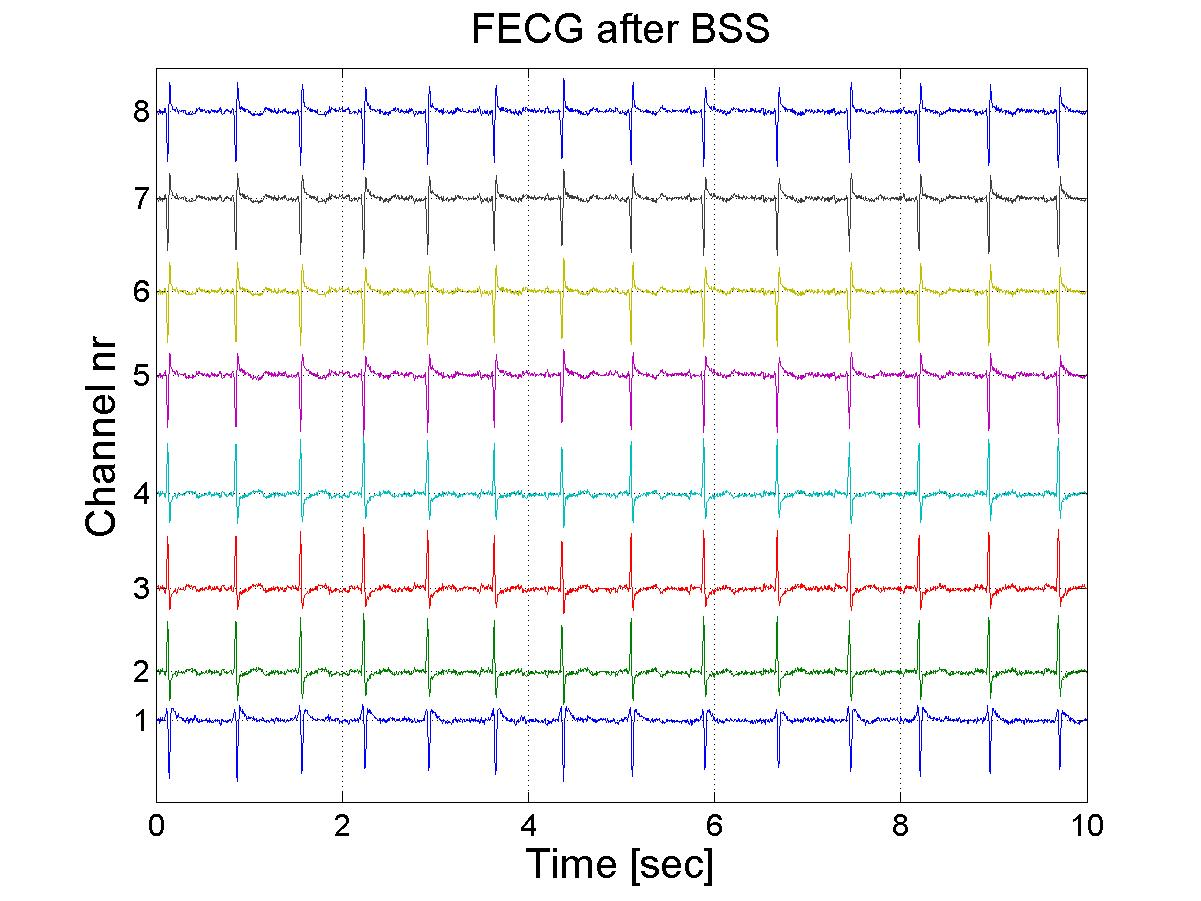
\includegraphics[width=1\linewidth]{101.jpg}
\subcaption{RRE estimation}\label{RRE1}
\endminipage\hfill
\minipage{0.33\textwidth}%
\centering
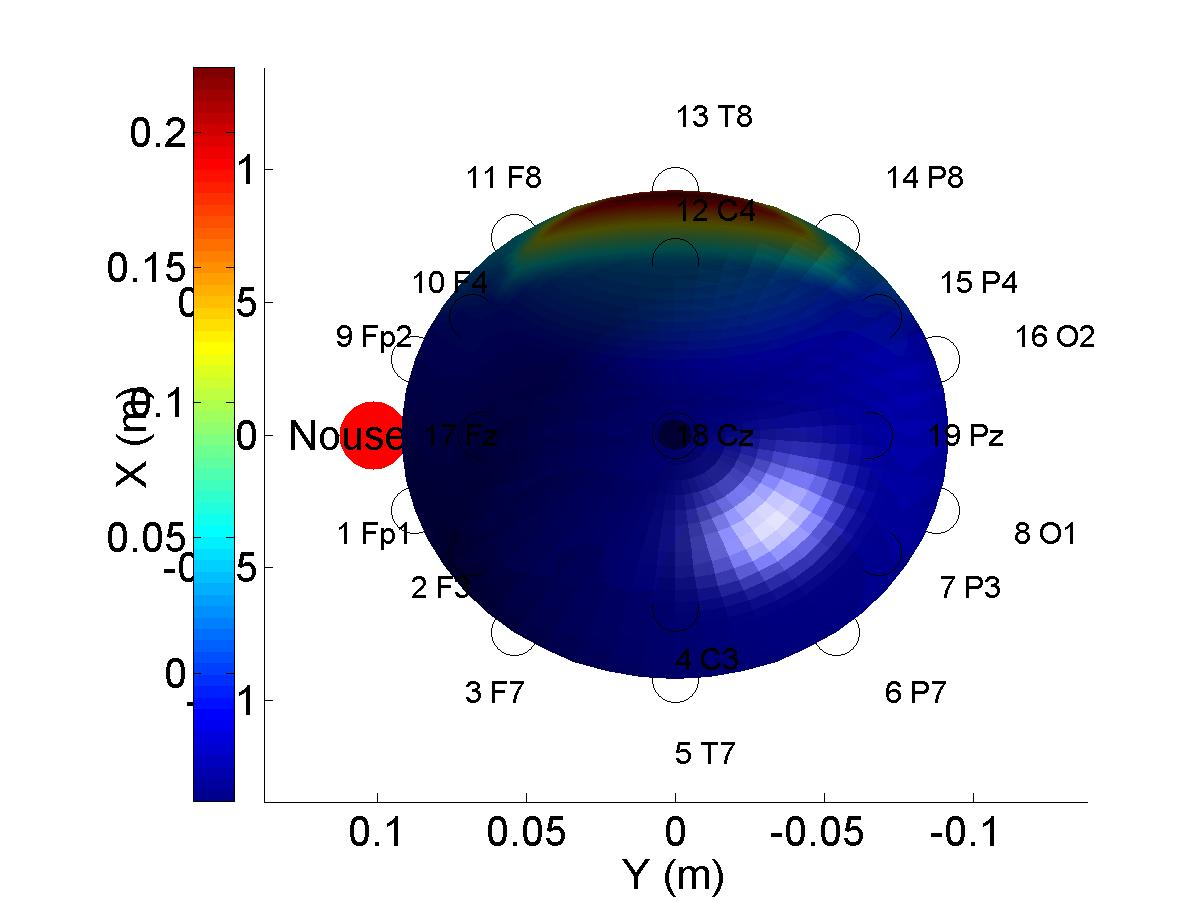
\includegraphics[width=1\linewidth]{102.jpg}
\subcaption{Voltage distribution to be used.}\label{VO1}
\endminipage\hfill
\caption{Inverse problem for a dipole located at (0.06,0,0) oriented along x}
\end{figure}



\subsection{Estimation of a dipole using the simulated EEG}


Hereby a certain potential is read from the simulated EEG in figure \ref{EEG} and the via inverse model the dipole is located from this particular time instance of the EEG. In the table \ref{Ta3} are the dipole locations data for this particular implementation.


\begin{table}[!htbp]
\centering
\caption{Inverse problem with electrode position altered}\label{Ta3}
\begin{tabular}{c c c c c c c c c c c c c c c c c c c c c c c c c c c c c c c }
\hline 
$ $&$X$&$Y$&$Z$&$OriX$&$OriY$&$OriZ$&$RRE$\\
\hline
\input{Files/EEG.txt} 
\hline 
\end{tabular}
\end{table}


\newpage
\subsection{Error due to not incorporating a malfunctioning electrode}

Hereby the importance of electrode functioning is verified. Using a dipole located at (0.06,0,0.01) oriented along x is used for this study. The potential distribution when all the electrodes are working is in figure \ref{VO2}, when the electrode P8 is off the potential distribution is as in the figure \ref{VO3} whereas when the electrod F7 is off the potential distribution is as in the figure \ref{VO4}
\begin{figure}[!htbp]
\minipage{0.33\textwidth}%
\centering
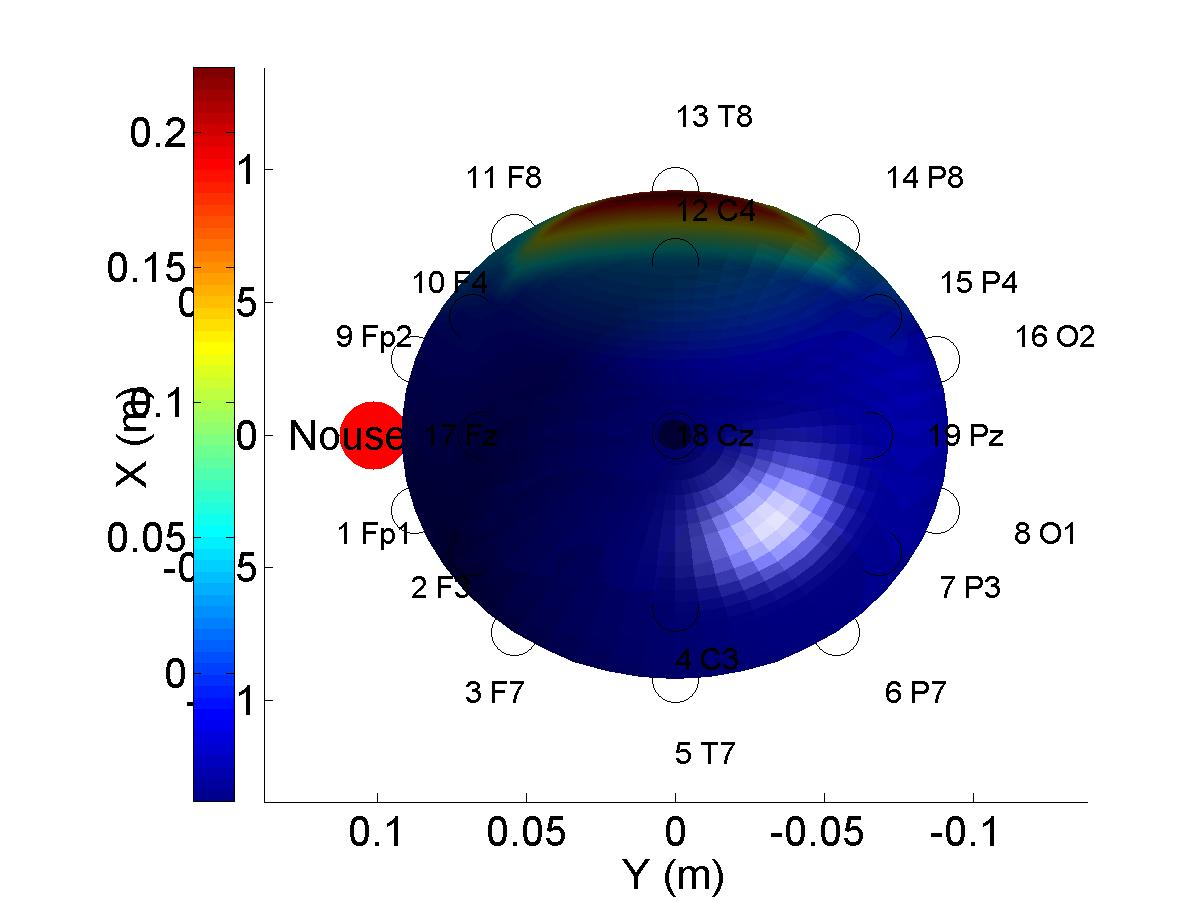
\includegraphics[width=1\linewidth]{103.jpg}
\subcaption{All the electrodes are working.}\label{VO2}
\endminipage\hfill
\minipage{0.33\textwidth}%
\centering
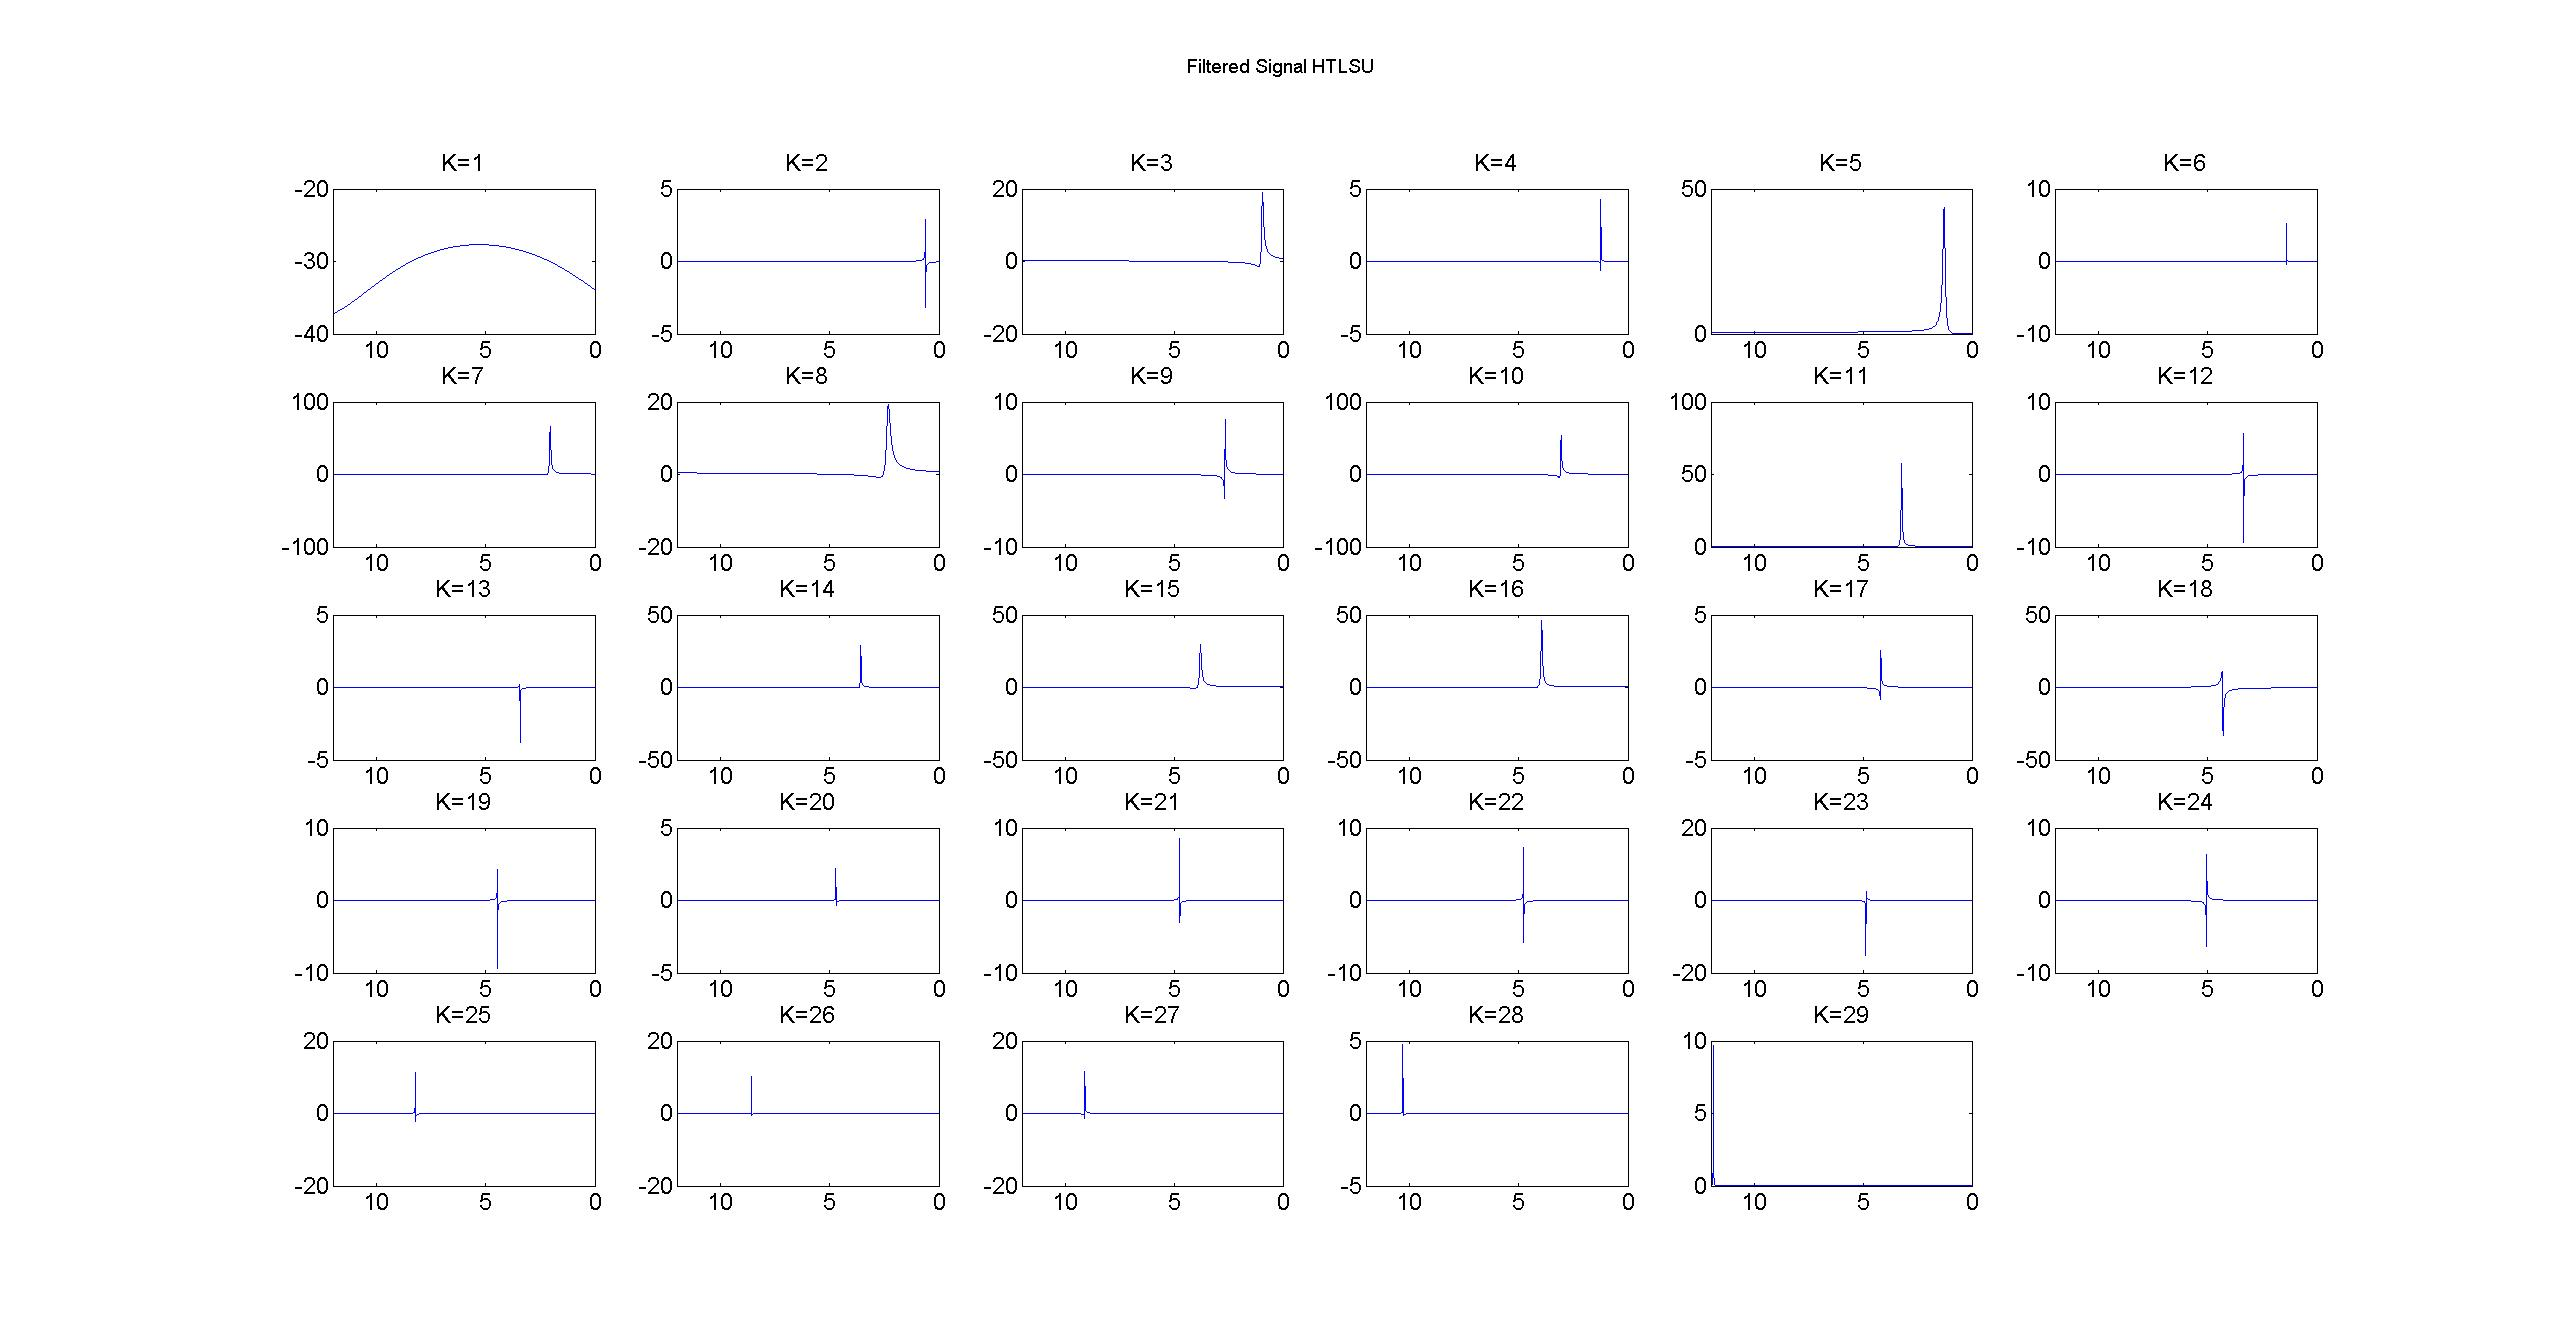
\includegraphics[width=1\linewidth]{104.jpg}
\subcaption{P8 is off.}\label{VO3}
\endminipage\hfill
\minipage{0.33\textwidth}%
\centering
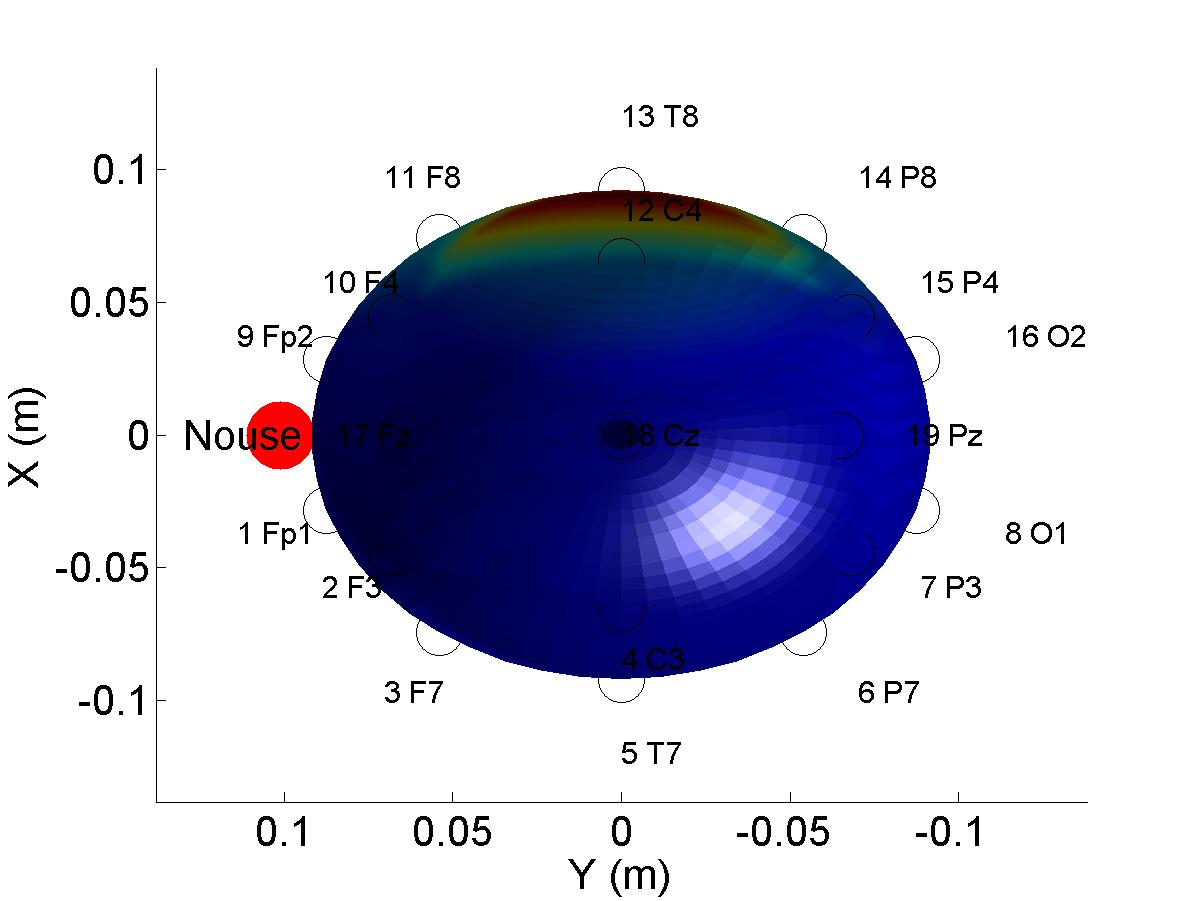
\includegraphics[width=1\linewidth]{105.jpg}
\subcaption{F7 is off.}\label{VO4}
\endminipage\hfill
\caption{Voltage distribution measurement}
\end{figure}


The inverse problem is applied in all these three cases. DOE and DLE plots for respective method are outlined in figure \ref{EEE}. As it is excepted these error are at lower scale for the case of full electrode well functioning \ref{EE2} whereas for the P8 case these errors are significantly higher campare to the F7 case respectively in figure \ref{EE3} and \ref{EE4}. At similiar figure is also the RRE plots in figure \ref{RRE2} where is is easitly observed the scale of error for the P8 case as compare to the F7 case. This is as a result that the P8 electrode location. This electrode is right in front of the main stream of the potential consequently being responsible for most flow. This flow is high in this direction due to the dipole orientation. Since the P8 is not functioning the potential measurement is measured dramatically wrong in this case. 

\begin{figure}[!htbp]
\minipage{0.33\textwidth}%
\centering
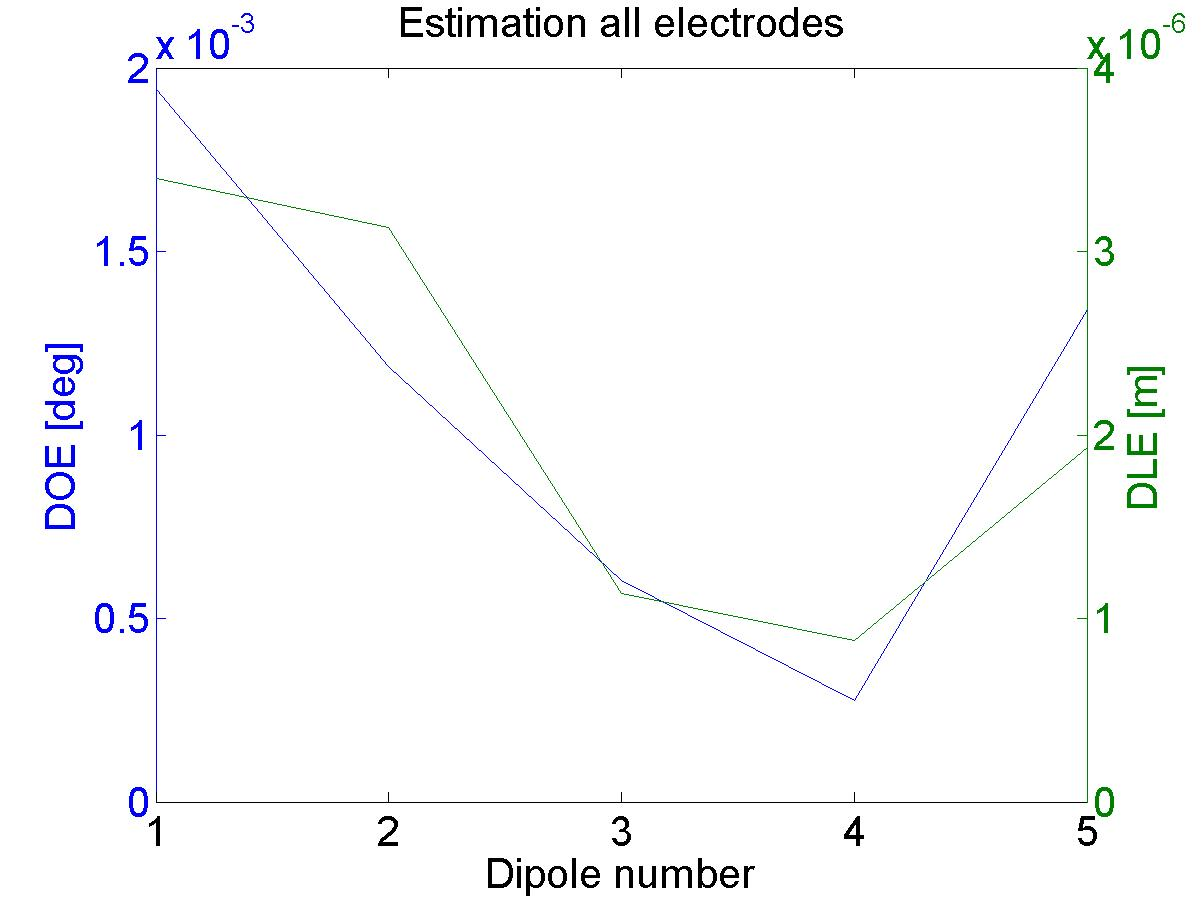
\includegraphics[width=1\linewidth]{107.jpg}
\subcaption{All the electrodes are working}\label{EE2}
\endminipage\hfill
\minipage{0.33\textwidth}%
\centering
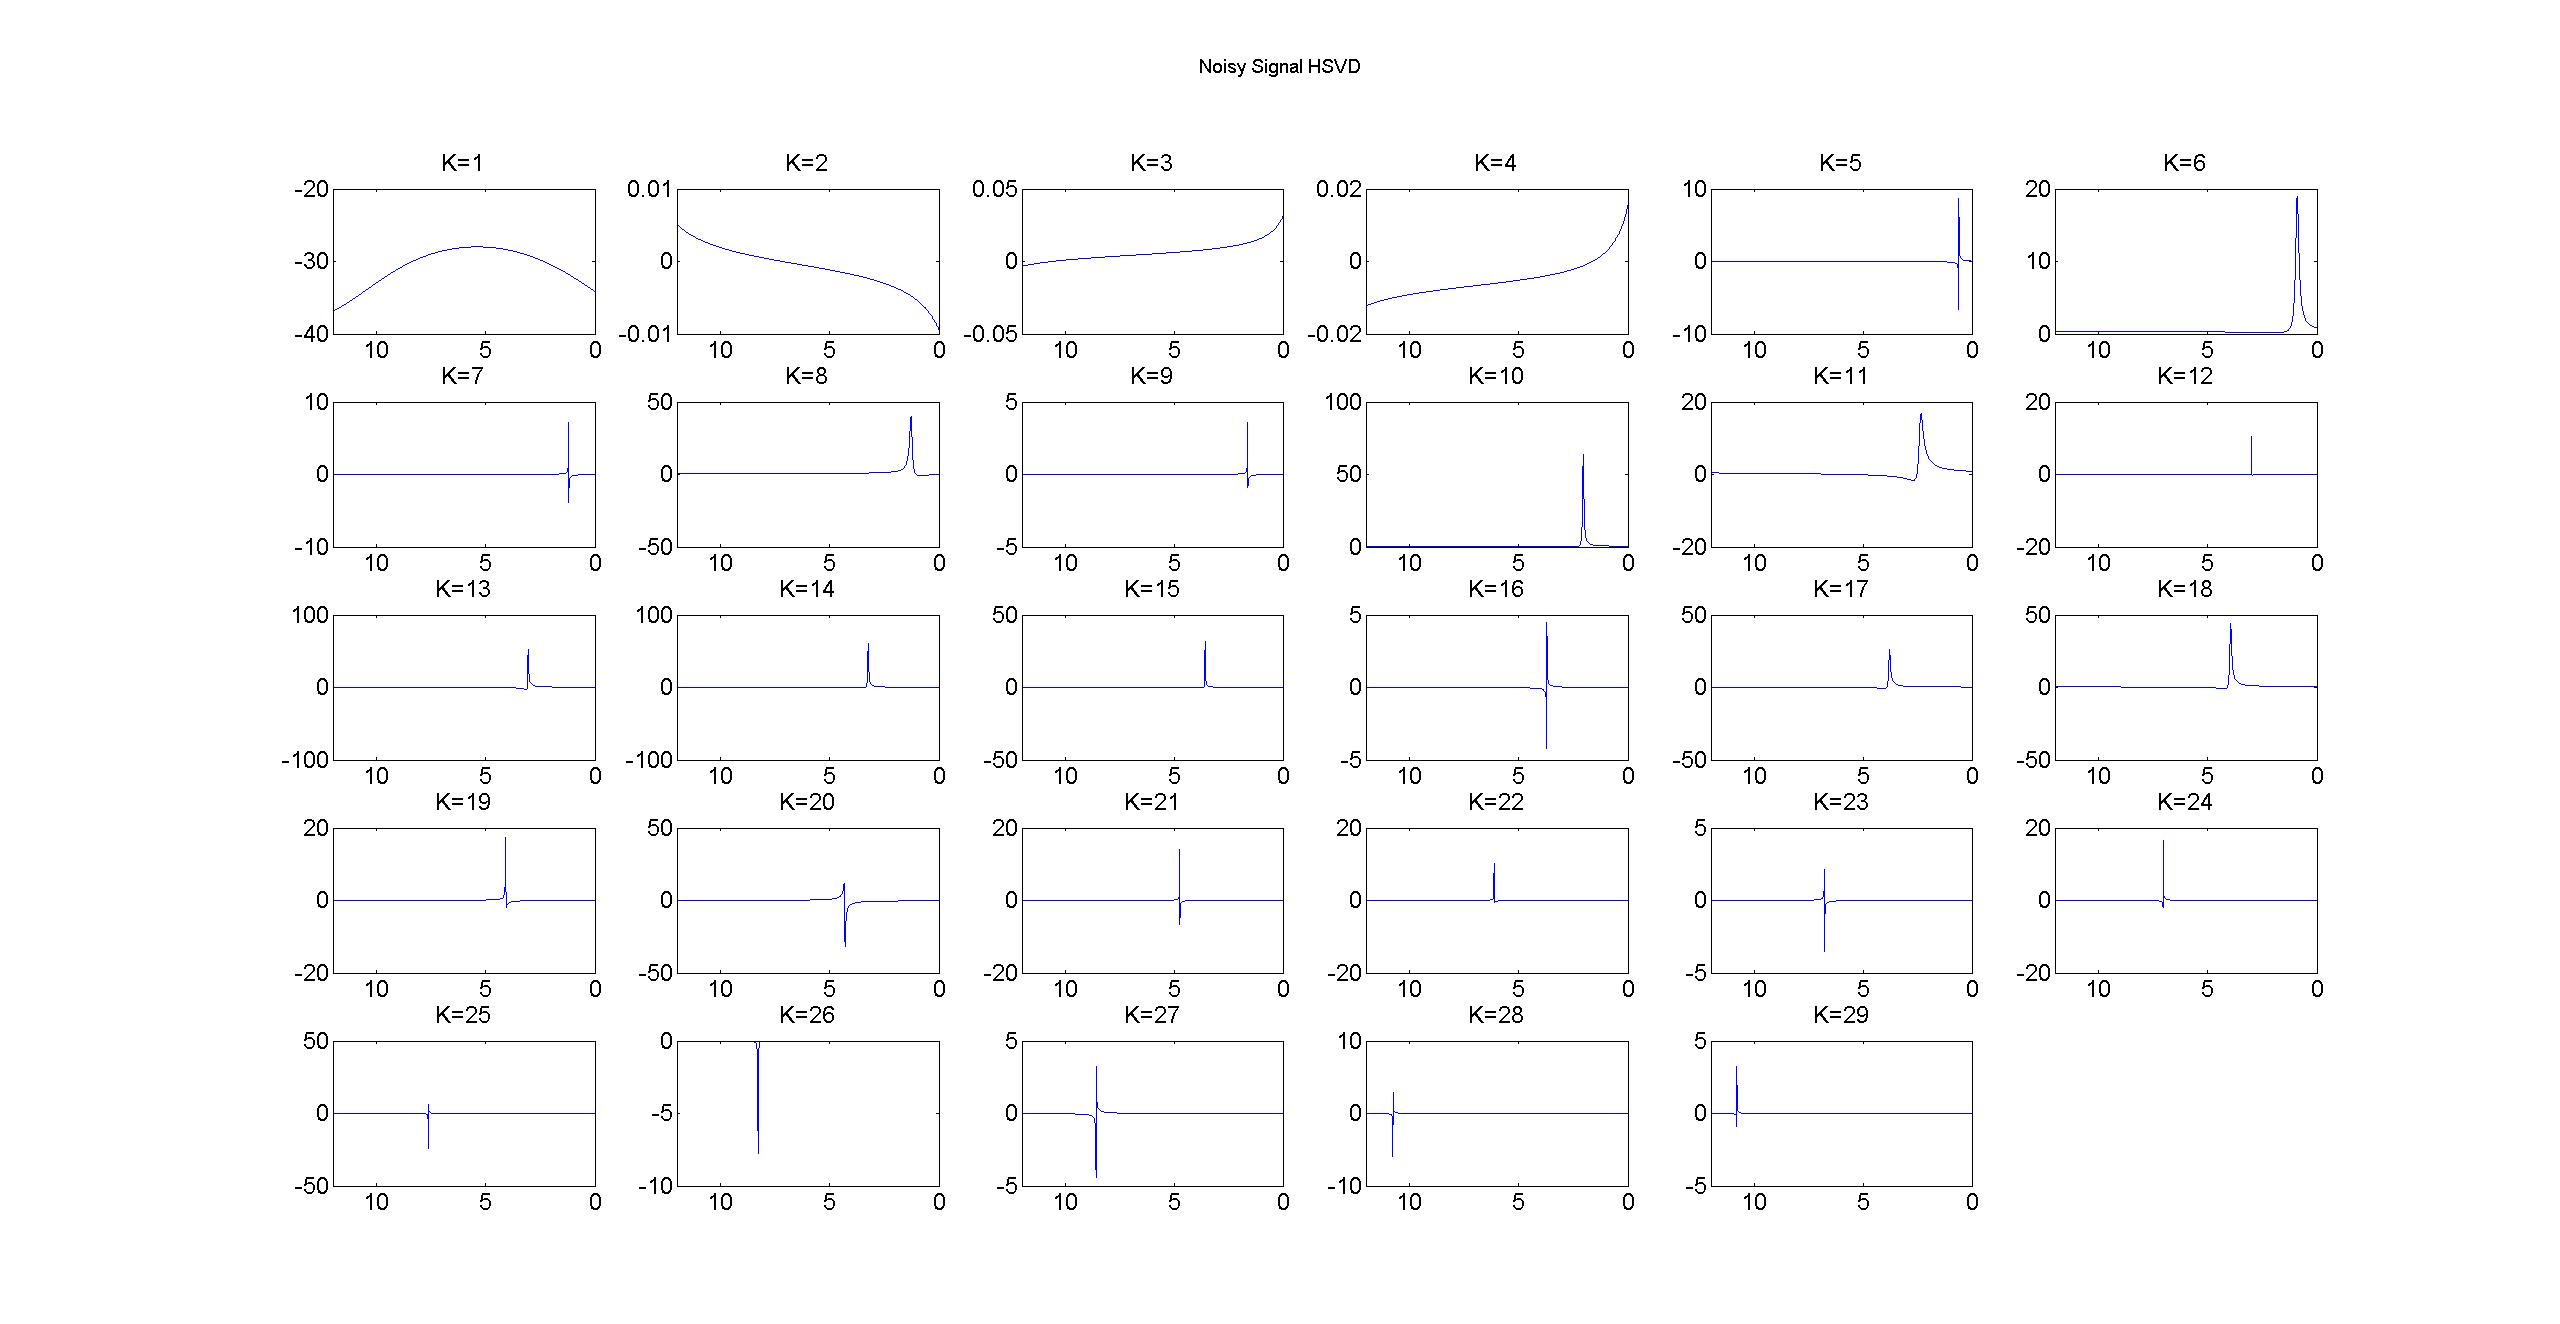
\includegraphics[width=1\linewidth]{108.jpg}
\subcaption{P8 electrodes is off}\label{EE3}
\endminipage\hfill
\minipage{0.33\textwidth}%
\centering
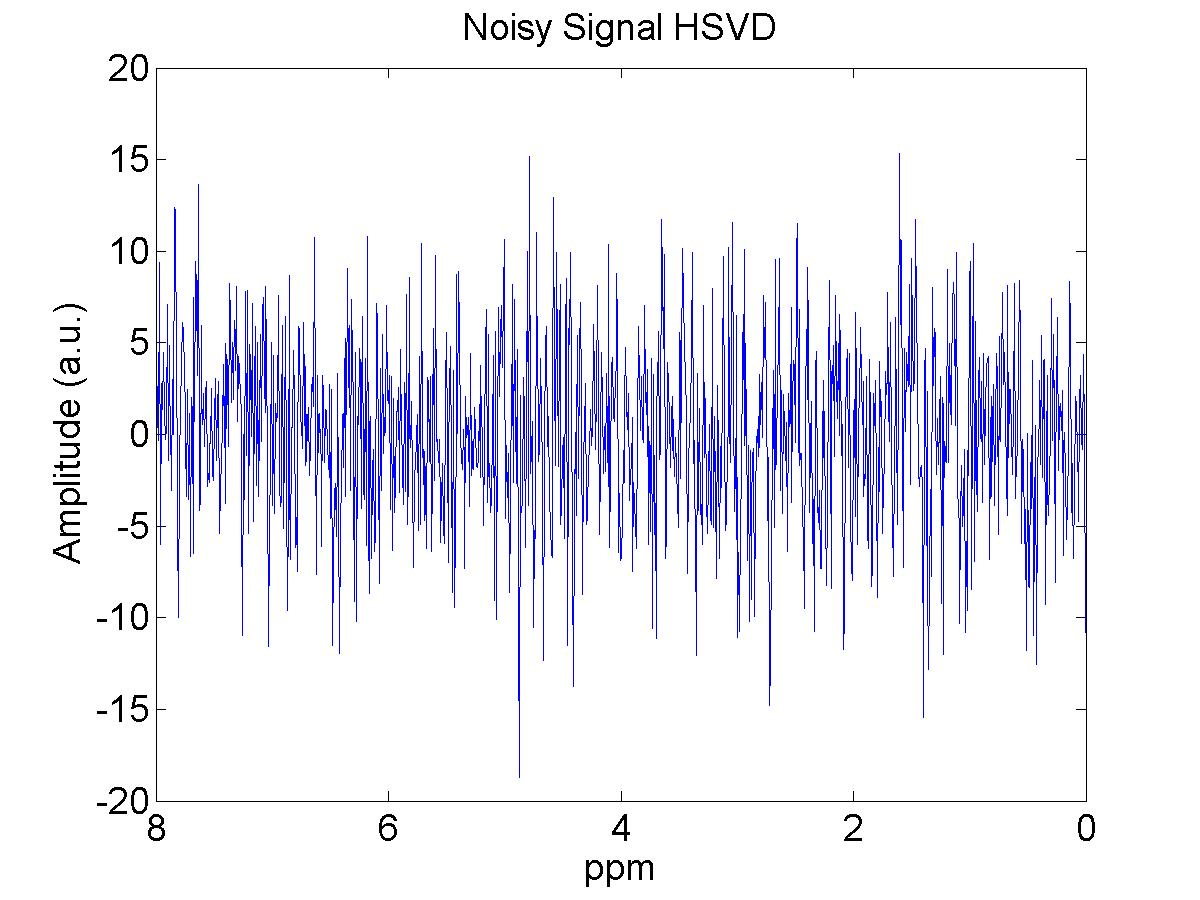
\includegraphics[width=1\linewidth]{109.jpg}
\subcaption{F7 electrodes is off}\label{EE4}
\endminipage\hfill
\caption{Localisation error for the three cases}\label{EEE}
\end{figure}

\begin{figure}[!htbp]
\centering
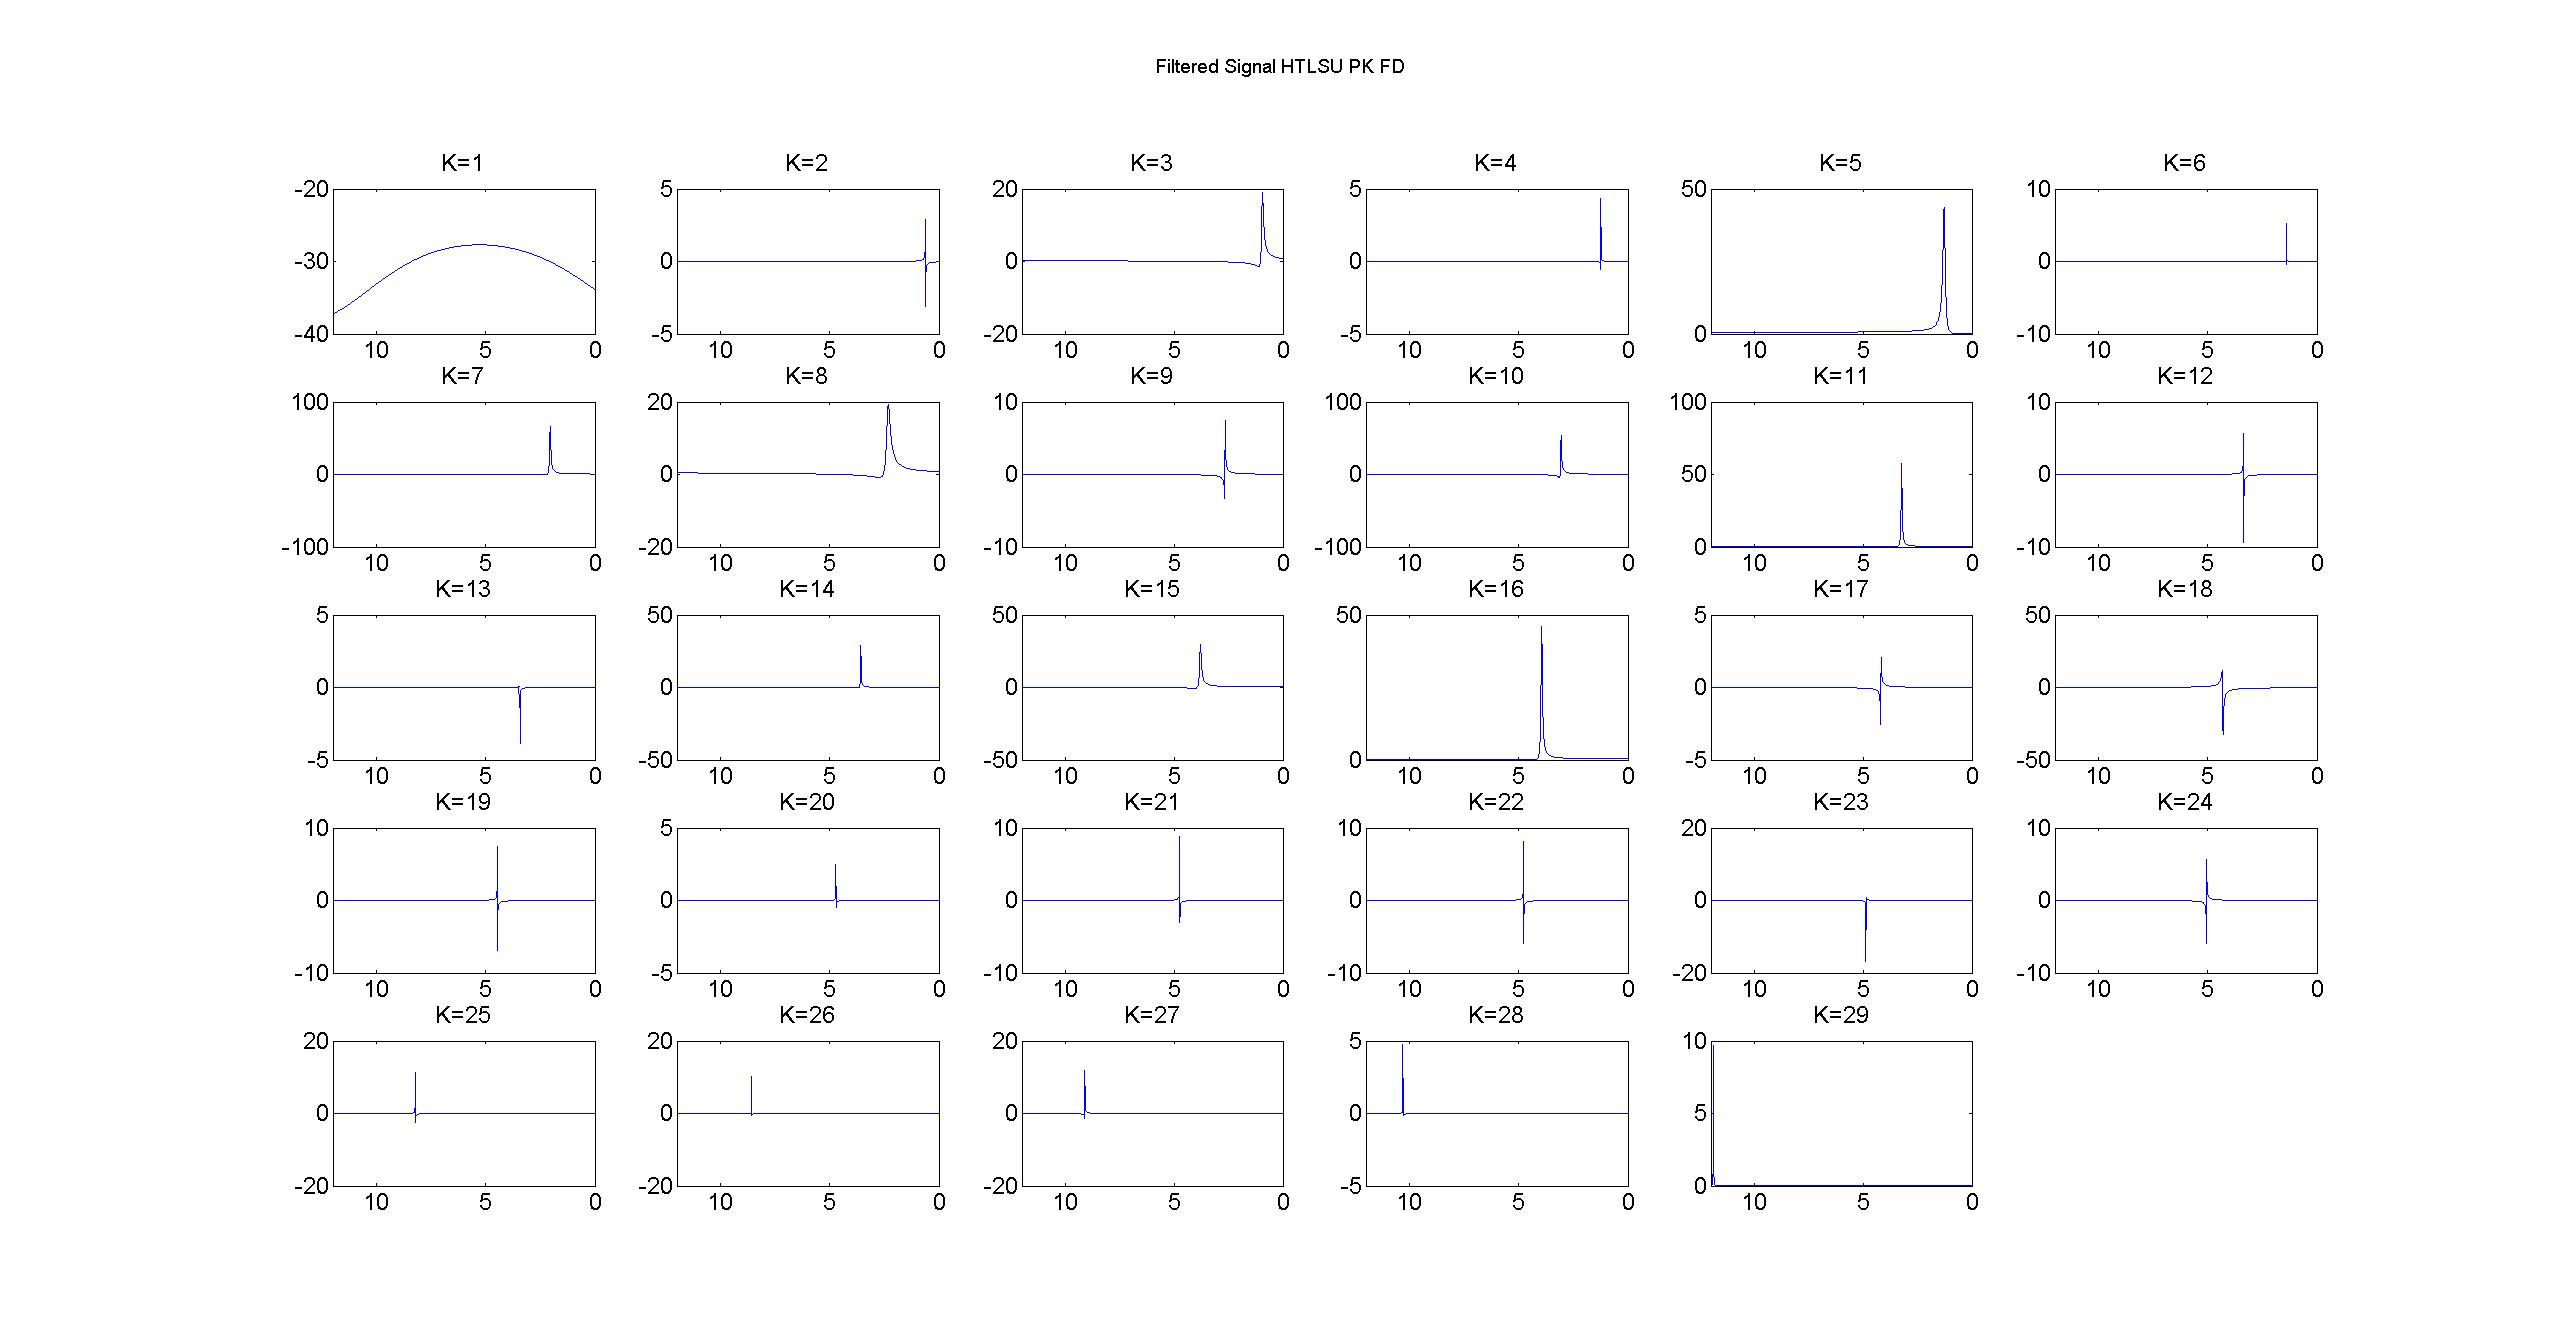
\includegraphics[width=0.35\linewidth]{106.jpg}
\caption{RRE estimation for the three cases}\label{RRE2}
\end{figure}


\newpage
\subsection{Error by different conductivity of the tissues}

Skull conductivity is also an important parameter for the inverse model. Hereby an experimental study is being conducted where the inverse problem is being uplied over a head model with different skull conductivity as compare to the head model where the forward problem is being computed. Hereby 10 different dipole are being tested where 5 different trials are tested for each dipole in the inverse problem. In the table \ref{Ta1} the solution are listed where Trial1D1 stands for trial 1 dipole 1. Whereas the DOE and DLE are plotted respectively in table \ref{Ta11} and \ref{Ta12} for each dipole trial over five different estimation for each trial. 

 \begin{table}[!htbp]
\centering
\caption{Inverse problem with skull conductivity altered}\label{Ta1}
\begin{tabular}{c c c c c c c c c c c c c c c c c c c c c c c c c c c c c c c } 
\hline 
$ $&$X$&$Y$&$Z$&$OriX$&$OriY$&$OriZ$&$RRE$\\
\hline
\input{Files/Skull.txt}
\hline 
\end{tabular}
\end{table}


\begin{table}[!htbp]
\centering
\caption{DOE for skull}\label{Ta11}
\begin{tabular}{c c c c c c c c c c c c c c c c c c c c c c c c c c c c c c c }
\hline 
$ $&$D1$&$D2$&$D3$&$D4$&$D5$\\
\hline
\input{Files/Skull1.txt} 
\hline 
\end{tabular}
\end{table}

\begin{table}[!htbp]
\centering
\caption{DLE for skull}\label{Ta12}
\begin{tabular}{c c c c c c c c c c c c c c c c c c c c c c c c c c c c c c c }
\hline 
$ $&$D1$&$D2$&$D3$&$D4$&$D5$\\
\hline
\input{Files/Skull2.txt} 
\hline 
\end{tabular}
\end{table}

In case the skull conductivity is not given the setup in figure \ref{new_label2} could be utilized for a particular measurement. 

\newpage
\subsection{Inverse problem with electrode position altered}

Similarly to the case when the skull conductivity was changed hereby a altering in the electrode position is performed. In table \ref{Ta2} are the result listed accordingly. Whereas the DOE and DLE are plotted respectively in table \ref{Ta21} and \ref{Ta22} for each dipole trial over five different estimation for each trial. The spherical angle is changed as in equation \ref{equation_3} for a particular displacement.


\begin{table}[!htbp]
\centering
\caption{Inverse problem with electrode position altered}\label{Ta2}
\begin{tabular}{c c c c c c c c c c c c c c c c c c c c c c c c c c c c c c c }
\hline 
$ $&$X$&$Y$&$Z$&$OriX$&$OriY$&$OriZ$&$RRE$\\
\hline
\input{Files/Electrode.txt} 
\hline 
\end{tabular}
\end{table}



\begin{table}[!htbp]
\centering
\caption{DOE for electrode misplacement}\label{Ta21}
\begin{tabular}{c c c c c c c c c c c c c c c c c c c c c c c c c c c c c c c }
\hline 
$ $&$D1$&$D2$&$D3$&$D4$&$D5$\\
\hline
\input{Files/Electrode1.txt} 
\hline 
\end{tabular}
\end{table}

\begin{table}[!htbp]
\centering
\caption{DLE for electrode misplacement}\label{Ta22}
\begin{tabular}{c c c c c c c c c c c c c c c c c c c c c c c c c c c c c c c }
\hline 
$ $&$D1$&$D2$&$D3$&$D4$&$D5$\\
\hline
\input{Files/Electrode2.txt} 
\hline 
\end{tabular}
\end{table}

As it could be noted, the error due to the electrode displacement sits at much higher values as compare to the case when the skull conductivity is changed. This infer a great importance of electrode placement in source localisation via inverse methods.